\documentclass[./main.tex]{subfiles}

\begin{document}

La fase di import è l'operazione che consiste nell'acquisizione dei dati dalle sorgenti e nella loro elaborazione al fine di renderli utilizzabili dall'applicazione.\par

\paragraph{Sorgenti di dati pubbliche.}
I dati pubblici riguardano le osservazioni da satellite e i radar. Questi dati sono tutti contenuti in cataloghi THREDDS. L'accesso ad essi può avvenire tramite diversi protocolli (vedi lista in \autoref{fig:access_tirlig}), quelli di interesse per \textit{Ismar Data} sono \textbf{WMS} e \textbf{NetcdfSubset}.
\begin{figure}[!ht]
\noindent\begin{minipage}{0.5\textwidth}
\vspace{1cm}
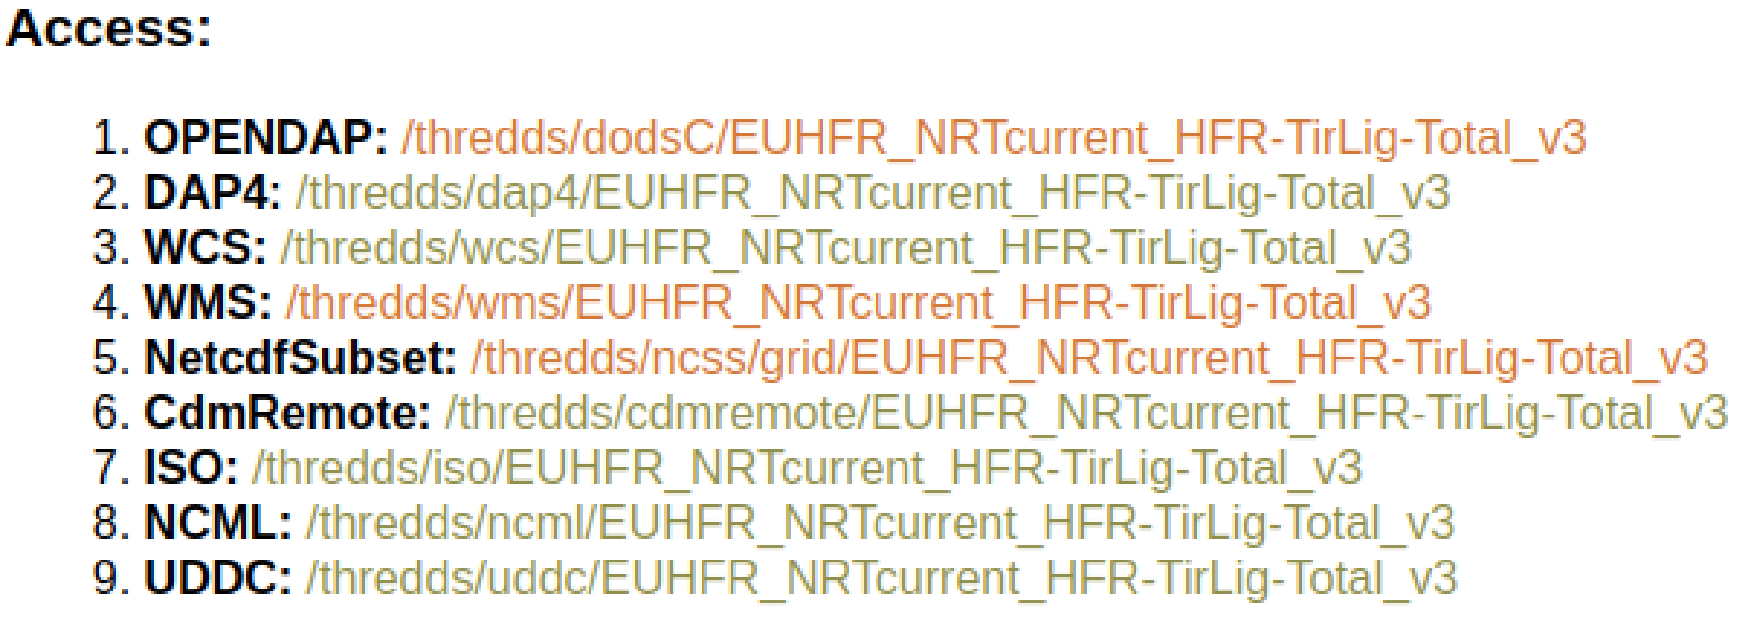
\includegraphics[width=\textwidth]{images/dataset_access.pdf}
\captionsetup{font=small, hypcap=false}
\captionof{figure}{Accesso dati HFR-TirLig\footcite[Fonte: ][\url{https://thredds.hfrnode.eu:8443/thredds/NRTcurrent/HFR-TirLig/HFR-TirLig_catalog.html?dataset=EUHFR_NRTcurrent_HFR-TirLig-Total_v3}]{thredds-hfr-trilig}.}
\label{fig:access_tirlig}
\end{minipage}
\hspace{0.05\textwidth}
\begin{minipage}{0.4\textwidth}
\begin{small}
Lista di protocolli per l'accesso ai dati del catalogo thredds della rete HFR-TirLig. I dataset di CHLa e SST hanno a disposizione solo OPENDAP, WMS e NetcdfSubset.
\end{small}
\end{minipage}
\vspace{0.25cm}
\end{figure}

Tutti i protocolli sono basati sull'architettura client-server. Lo schema classico del modello è presente in \autoref{fig:client_server_model}.
\begin{figure}[!ht]
\noindent\begin{minipage}{0.5\textwidth}
\vspace{1cm}
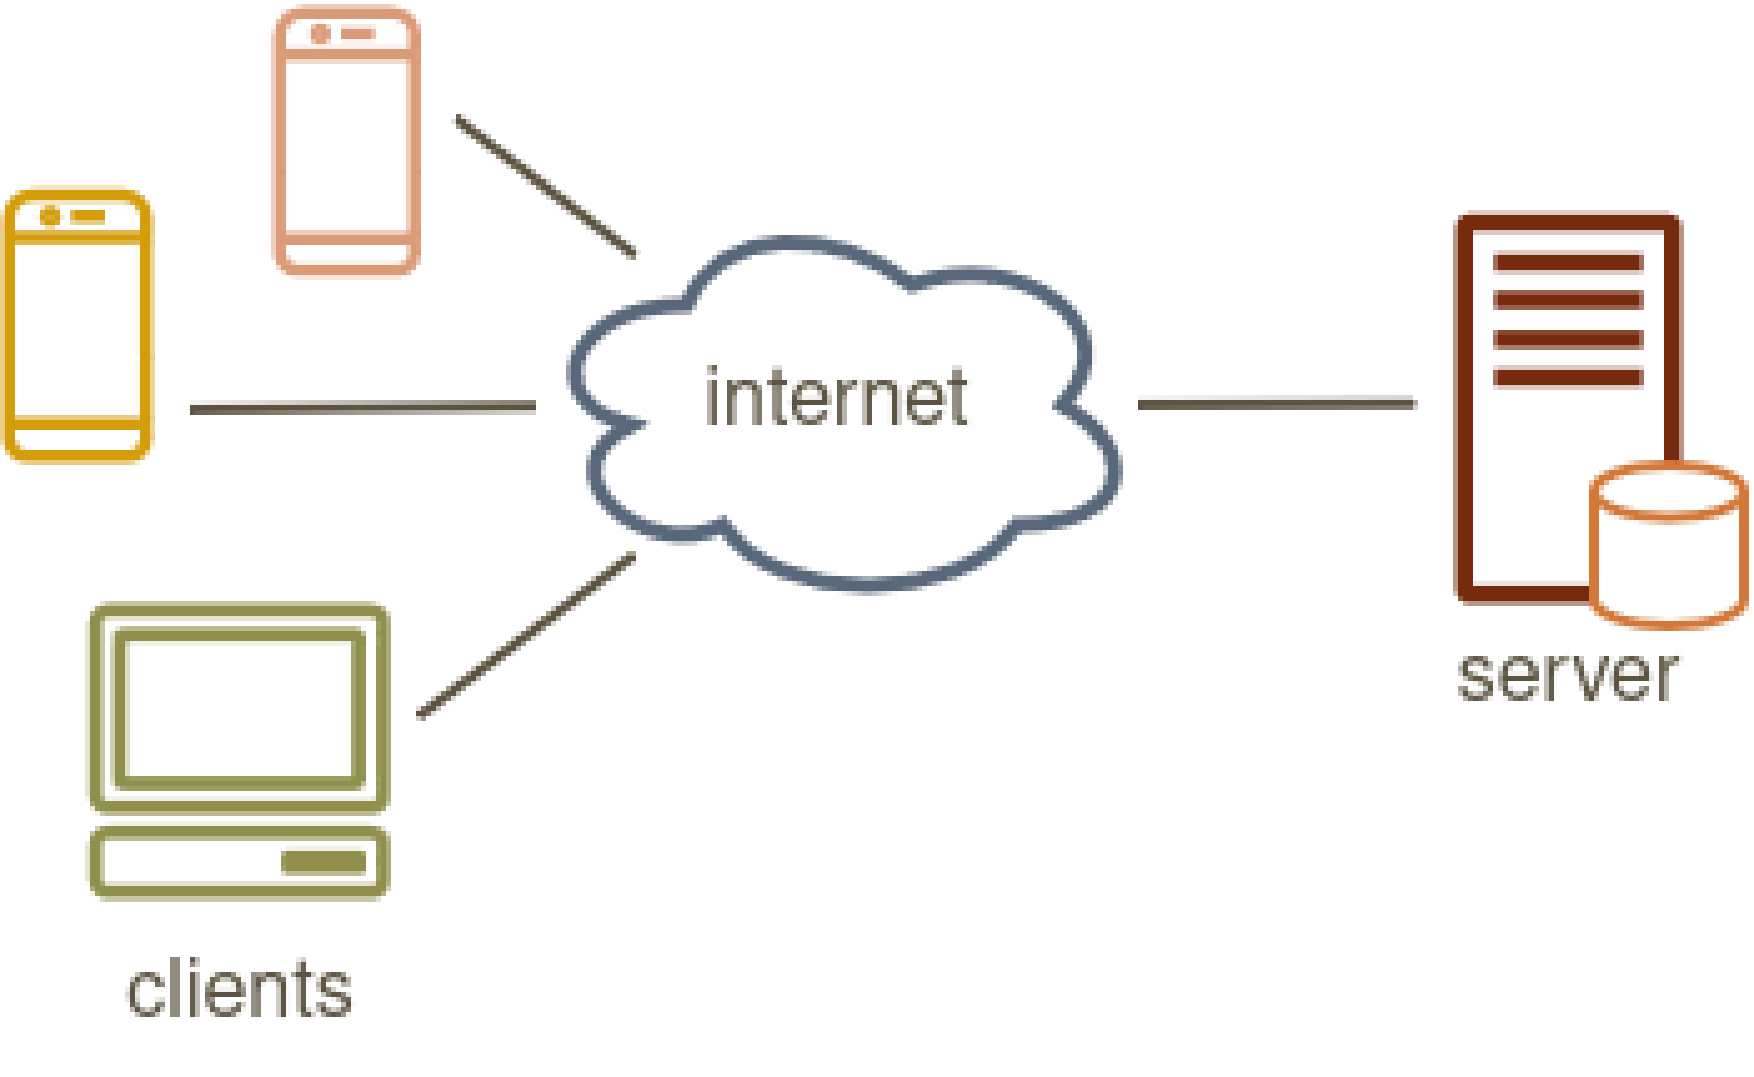
\includegraphics[width=\textwidth]{images/client-server-model.pdf}
\captionsetup{font=small, hypcap=false}
\captionof{figure}{Modello client-server (Diagramma creato utilizzando drawio\footcite[\url{https://www.drawio.com/}]{website-drawio}.).}
\label{fig:client_server_model}
\end{minipage}
\hspace{0.05\textwidth}
\begin{minipage}{0.4\textwidth}
\begin{small}
Schema classico del modello client-server dove essi comunicano attraverso la rete. 
\end{small}
\end{minipage}
\vspace{0.25cm}
\end{figure}
Questa architettura descrive un modello nel quale un computer, detto client, richiede delle risorse a un altro elaboratore, chiamato server, attraverso una connessione di rete. Il server riceve la richiesta, la elabora e risponde al client. Potrebbe accadere che ci siano più elaboratori, sia da un lato che dall'altro. Inoltre, spesso allo schema base viene aggiunto un database dove il server conserva dati e informazioni. L'architettura client-server è uno dei modelli più utilizzato quando si tratta di richieste nelle quali compaiano i due attori\footcite[139-142]{clientServerModel}.\par

Il \textbf{WMS} (\textit{Web Map Service Interface Standard}) fornisce mappe di dati con riferimenti spaziali in modo dinamico a partire da informazioni geografiche. Per mappa non si intende i dati veri e propri, ma una rappresentazione sotto forma di immagine digitale adatta ad essere visualizzata in uno schermo. Questa immagine può essere in formato pdf, GIF o JPEG, o addirittura SVG (\textit{Scalable Vector Graphics})\footcite[5]{ogc-wms-specs}. Sono possibili diverse operazioni, di cui due fondamentali. La prima \textit{GetCapabilities} serve ad ottenere metadati (i metadati sono informazioni strutturate che descrivono e rendono più facile l'accesso alle informazioni) sul servizio, insieme alle possibili operazioni e alla lista dei \textit{layer} disponibili. Ogni mappa disponibile è un layer con un nome a cui riferirsi. Per ottenere l'immagine della mappa si utilizza la seconda operazione \textit{GetMap}, specificando il layer e il formato nei parametri\footcite[21-38]{ogc-wms-specs}.\par

\textbf{NetCDF} -- \textit{network Common Data Form} -- è un modello per dati scientifici orientati agli array. Esistono diverse librerie distribuite gratuitamente che implementano il supporto a questo modello per la creazione, l'accesso e la condivisione dei dati. Le raccolte di dati create con NetCDF includono sempre informazioni su cosa contengono e sono accessibili velocemente da qualsiasi dispositivo. Inoltre, un archivio rende possibile l'accesso a tutte le versioni\footcite[7]{ogc-netcdf-specs} create.  Il modello classico rappresenta le informazioni scientifiche in un dataset netCDF usando dimensioni, variabili e attributi. Le variabili contengono i dati salvati come array multidimensionali aventi lo stesso tipo di forma. La forma è intesa come una lista da zero ad n dimensioni (0 rappresenta una variabile con un singolo valore, 1 rappresenta un vettore, 2 rappresenta una matrice, detta anche griglia, e così via fino ad N). Le dimensioni sono inoltre usate per le griglie comuni e per il sistema di coordinate. Gli attributi invece contengono metadati, ovvero informazioni sulle proprietà di una variabile o dell'intero dataset\footcite[10-15]{ogc-netcdf-specs}.\par

\textbf{NetCDF Subset Service }(\textit{NCSS}) è un servizio web per un sottoinsieme di dati NetCDF.  Gli array di dati vengono suddivisi in sottoinsiemi, specificano le coordinate terrestri (per es. utilizzando latitudine/longitudine) oppure intervalli di date, preservando comunque la risoluzione e l'accuratezza del set di dati originale. Un dataset in questo servizio corrisponde a un documento XML e fornisce abbastanza dettagli per rendere possibile una richiesta da parte del client. I dataset dei cataloghi thredds sono tutti una collezione di griglie. Ciò significa che hanno coordinate orizzontali (x ed y), opzionalmente anche verticali, hanno il tempo e un insieme di coordinate\footcite[\url{https://docs.unidata.ucar.edu/tds/current/userguide/netcdf_subset_service_ref.html}]{website-unidata-ucar-edu}. Nei cataloghi analizzati, la risposta del server produce un file netCDF4.\par

Dalla descrizione si evidenzia come il formato WMS sia particolarmente comodo per ottenere un'immagine senza troppi sforzi, mentre netCDFsubset necessita del salvataggio di un file contenente l'intero dataset che deve poi essere elaborato per produrre un qualcosa di concreto. Contrariamente a quanto sembra, netCDFsubset è la scelta migliore. Questo perché, tramite la libreria \textbf{gdal} (\textit{Geospatial Data Abstraction Library}),  disponibile anche per Python, è possibile tradurre facilmente i formati di dati geospaziali\footcite[\url{https://gdal.org/}]{gdal-docs}. WMS non è però da escludere, infatti viene momentaneamente utilizzato per plottare\footnote{\textbf{plottare}  v. tr. [adattam. dell’ingl. (\textit{to}) \textit{plot} «tracciare una mappa, un piano», con influsso diretto di \textit{plotter}]. – Nel gergo anglicizzante dell’informatica, disegnare, tracciare un diagramma mediante il \textit{plotter}; \cite{treccani-plottare}.} i dati nella demo web.\par

%\paragraph{Implementazione.} 
Le funzioni che si occupano di interagire con il server dei cataloghi thredds e della elaborazione dei dati raccolti, seguono il principio del riuso del codice, sfruttando ciò che già esiste per tutti i cataloghi (radar, Chla, SST). Ora che questo è chiaro si può procedere all'analisi dell'implementazione dell'import, prima netCDFsubset e in seguito WMS\par

La procedura \textit{"etl"} in \autoref{lst:etl_urls} contiene tutte le funzionalità per scaricare i dati dai cataloghi e convertirli tramite gdal. Inizialmente quindi i dati sono scaricati dal catalogo con una funzione (vedi \autoref{lst:etl_download_netcdf}) che, dato il link al file netCDF sul server, lo scarica in una cartella predefinita, controllando che il server dia un codice di risposta positivo.

\begin{lstlisting}[language=Python, 
    caption={Procedura utilizzata per scaricare e convertire i dati dei cataloghi thredds.},
    label=lst:etl_urls]
    def etl(day: str, dataset: str, variable: str, add_variable_to_filepath: bool = False):
    ...
    # url for each thredds catalog
    # ncss protocol used
    # accept=netcdf output format
    # download dai cataloghi thredds
    if dataset == "sst":
        url = f"http://ritmare.artov.ismar.cnr.it/thredds/ncss/sstuhr?var=\{variable\}\&disableLLSubset=on\&disableProjSubset=on\&horizStride=1\&time=\{day\}\&addLatLon=true\&accept=netcdf"
    elif dataset == "chl":
        url = f"http://ritmare.artov.ismar.cnr.it/thredds/ncss/xchlcase12?var=\{variable\}\&disableLLSubset=on\&disableProjSubset=on\&horizStride=1\&time=\{day\}\&addLatLon=true\&accept=netcdf"
    elif dataset == "hfr":
        url = f"https://thredds.hfrnode.eu:8443/thredds/ncss/EUHFR\_NRTcurrent\_HFR-TirLig-Total\_v3?var=\{variable\}\&north=44.4960\&west=7.5069\&east=10.4930\&south=43.2539\&disableLLSubset=on\&disableProjSubset=on\&horizStride=1\&time=\{day\}\&vertCoord=0"
    else:
        logging.error(f"Wrong input as dataset: \{dataset\}")
        raise ValueError()   

    print(f"URL: {url}")
    temp_path = tempfile.gettempdir() + f"/{dataset}_{day}.nc"

    try:
        # scaricamento file netcdf nella cartella
        download_successful = download_netcdf(url, temp_path)
        if not download_successful:
            raise DownloadError("Download failed.")

        if add_variable_to_filepath:
            destination_path = os.path.join(
                BASE_DIR, "ismarbo/static/ismarbo/thredds", dataset, variable
            )
        else:
            destination_path = os.path.join(
                BASE_DIR, "ismarbo/static/ismarbo/thredds", dataset
            )
        timestamp = get_time(temp_path)

        destination_file = os.path.join(
            destination_path,
            f"{timestamp}.tif",
        )

        # conversione dati tramite gdal
        conversion_successful = convert_nc_to_geotiff(
            temp_path,
            destination_file,
            variable,
        )

        if not conversion_successful:
            raise ConversionError("Conversion failed.")

        return timestamp

    except (DownloadError, ConversionError, DatabaseLoadError, ValueError) as e:
        logging.error(f"Process terminated: {e}")

    logging.info("All operations completed successfully.")
\end{lstlisting}

\begin{lstlisting}[language=Python, 
    caption={Definzione funzione per scariare in local un file netCDF dato il link al server.},
    label=lst:etl_download_netcdf]
    def download_netcdf(url, temp_path)
\end{lstlisting}

Successivamente avviene l'operazione principale: la conversione dei file netcdf ottenuti in formato \textbf{GeoTIFF}  (\textit{Geographic Tagged Image File Format}) tramite gdal. Per comprendere cosa sia GeoTIFF occorre analizzare \textbf{TIFF}. TIFF (\textit{Tagged Image File Format}) è un formato di file basato su tag per salvare immagini (in bianco e nero, in scala di grigi e a colori) raster. Data la sua indipendenza dall'architettura del computer, sia lato software che lato hardware, e la sua adattabilità ad essere aperto da qualsiasi programma, è molto utilizzato. GeoTIFF è quindi definito come un insieme di tag TIFF che descrivono tutte le informazioni geografiche, in questo modo i dati possono essere collegati a una proiezione di una mappa\footcite[1-4]{tiff-geotiff}. Tutto questo viene fatto all'interno della funzione \textit{"convert\_nc\_to\_geotiff"} (vedi \autoref{lst:convert_nc_to_geotiff}) che, dato il file netcdf, il percorso in cui salvare il risultato ottenuto, la variabile di interesse (per i dataset composti da più variabili, come i radar), e il sistema di coordinate standard utilizzato, converte il dataset di partenza in geoTIFF attraverso:
\begin{itemize}
    \item \lstinline[language=Python]{gdal.Open(nc_file)}
    : apre un dataset netCDF\footcite[\url{https://gdal.org/tutorials/raster_api_tut.html\#opening-the-file}]{gdal-docs};
    \item \lstinline[language=Python]{gdal.Translate(output_tiff, nc_dataset, options=translate_options)}
    : converte il dataset in formato geoTIFF, salvando il file TIFF\footcite[\url{https://gdal.org/programs/gdal_translate.html\#gdal-translate}]{gdal-docs}.
\end{itemize}

\begin{lstlisting}[language=Python, 
    caption={Definzione funzione per la conversione dei file netCDF in geoTIFF.},
    label=lst:convert_nc_to_geotiff]
    def convert_nc_to_geotiff(nc_file, output_tiff, variable_name=None, band=1, crs="EPSG:4326")
\end{lstlisting}

L'ultima importante funzione \textit{"load\_geotiff\_to\_postgis"} (vedi \autoref{lst:load_geotiff_to_postgis}) è quella che consente di salvare i dati GeoTIFF nel database postgreSQL utilizzando le funzionalità offerte dal plugin postGIS. Al momento è stata solamente progettata per usi futuri, appena sarà chiaro se salvare tutto (dati statici e dinamici) all'interno dello stesso database o se separare queste tipologie di dati.\par

\begin{lstlisting}[language=Python, 
    caption={Definzione funzione per il salvataggio dei dati GeoTIFF all'interno del database PostgreSQL.},
    label=lst:load_geotiff_to_postgis]
    def load_geotiff_to_postgis(geotiff_path, database, table, host="localhost", port=5432, user="your_username", password="your_password")
\end{lstlisting}

I dati devono essere aggiornati periodicamente, eliminando i vecchi dati e sostituendoli con gli ultimi disponibili.  Questo viene fatto tramite il meccanismo dei  \textbf{cron-job}. Cron è lo scheduler dei lavori basato sul tempo nei sistemi operativi Unix-like per consentire l'esecuzione di lavori -- \textit{job} -- periodicamente in determinati orari, date o intervalli\footcite[\url{https://wiki.archlinux.org/title/Cron}]{website-arch-wiki}. L'implementazione (vedi \autoref{lst:cron_jobs_thredds}) sul progetto è semplificata grazie a \textbf{django-cron} che evita la complicata costruzione di uno script Python apposito o l'utilizzo di un comando di gestione per cron (ancora peggio!)\footcite[\url{https://django-cron.readthedocs.io/en/latest/introduction.html}]{website-django-cron}. 

\begin{lstlisting}[language=Python, 
    caption={Definzione dei cron job per i dati dei cataloghi thredds. Lo scaricamento dei dati avviene chiamando le funzioni sst\_cron\_etl, chl\_cron\_etl e hfr\_cron\_etl, mentre l'elimanzione tramite le rispettive cleanup.},
    label=lst:cron_jobs_thredds]
    CRONJOBS = [
        (
            "0 5 * * *", # 5:00am
            "ismarbo.tasks.sst_cron_etl",
            f">> {BASE_DIR}/ismarbo/static/ismarbo/thredds/sst/logs/cronlogs.log 2>&1",
        ),
        (
            "30 5 * * *", # 5:30am
            "ismarbo.tasks.chl_cron_etl",
            f">> {BASE_DIR}/ismarbo/static/ismarbo/thredds/chl/logs/cronlogs.log 2>&1",
        ),
        (
            "4 */1 * * *", # al minuto 4 ogni ora
            "ismarbo.tasks.hfr_cron_etl",
            f">> {BASE_DIR}/ismarbo/static/ismarbo/thredds/hfr/logs/cronlogs.log 2>&1",
        ),
        (
            "0 3 * * *", # 3:00am
            "ismarbo.tasks.sst_cleanup",
            f">> {BASE_DIR}/ismarbo/static/ismarbo/thredds/sst/logs/cleanuplogs.log 2>&1",
        ),
        (
            "10 3 * * *", # 3:10am
            "ismarbo.tasks.chl_cleanup",
            f">> {BASE_DIR}/ismarbo/static/ismarbo/thredds/chl/logs/cleanup.log 2>&1",
        ),
        (
            "20 3 * * *", # 3:20am
            "ismarbo.tasks.hfr_cleanup",
            f">> {BASE_DIR}/ismarbo/static/ismarbo/thredds/hfr/logs/cleanup.log 2>&1",
        ),
    ]
\end{lstlisting}

L'accesso ai dati tramite protocollo WMS avviene solamente per la demo web grazie a \textbf{Leaflet}, un esempio è mostrato in \autoref{fig:demo_sst_chla}. Leaflet è una libreria JavaScript open-source per visualizzare mappe interattive in modo semplice e veloce. Inoltre supporta il sistema di coordinate utilizzato dai cataloghi, altrimenti non sarebbe di alcuna utilità\footcite[\url{https://leafletjs.com/index.html}]{website-leaflet}. Leaflet utilizza l'url base, ovvero senza indicare alcun metodo, del servizio WMS per creare una mappa. Specificando il layer di interesse e le varie opzioni si ottiene immediatamente l'immagine da visualizzare (vedi codice in \autoref{lst:leaflet_wms_sst} e \autoref{lst:leaflet_wms_chl}). Ai fini della visualizzazione, è importante notare che il nome del layer da utilizzare non è quello indicato dal documento XML GetCapabilites di WMS. Per ottenere il giusto nome del layer è consigliato utilizzare un qualsiasi programma di visualizzazione di WMS, come QGis\footcite[\url{https://leafletjs.com/examples/wms/wms.html}]{website-leaflet}. Ad esempio in \autoref{lst:leaflet_wms_sst} il nome del layer ottenuto tramite QGis risulta essere \textit{"analysed\_sst"}, mentre il nome indicato dal documento XML è\textit{"sst"}.


\begin{lstlisting}[language=javascript, caption={Utilizzo di Leaflet per ricavare l'immagine della mappa per la variabile SST, a cui saranno aggiunte funzionalità per l'interazione}, label=lst:leaflet_wms_sst]
    var overlayMaps = {
        "Sea Surface Temperature": L.tileLayer
            .wms("http://ritmare.artov.ismar.cnr.it/thredds/wms/sstuhr", {
                layers: "analysed_sst",
                format: "image/pdf",
                transparent: true,
                version: "1.3.0",
                attribution: "CNR THREDDS Catalog for RITMARE Project - Sea Surface Temperature",
                TIME: "2014-01-01T00:00:00.000Z",
            })
        ...
\end{lstlisting}

\begin{lstlisting}[language=javascript, caption={Utilizzo di Leaflet per ricavare l'immagine della mappa per la variabile Chla, a cui saranno aggiunte funzionalità per l'interazione}, label=lst:leaflet_wms_chl]
    ...
    Chlorophyll: L.tileLayer
        .wms("http://ritmare.artov.ismar.cnr.it/thredds/wms/xchlcase12", {
            layers: "CHL",
            format: "image/pdf",
            transparent: true,
            attribution: "CNR THREDDS Catalog for RITMARE Project - Chlorophyll",
            TIME: "2014-01-01T00:00:00.000Z",
        })
    ...
\end{lstlisting}


Il layer può poi essere sovrapposto ad una mappa base del territorio (vedi codice in \autoref{lst:leaflet_base}). Una mappa base è una mappa di riferimento alla quale è possibile sovrapporre più livelli di dati geografici, in particolare per la demo sono utilizzate quelle fornite da CARTO\footcite[\url{https://carto.com/basemaps}]{website-carto}. L'effetto di queste operazioni è mostrato in \autoref{fig:demo_sst_chla}, dove, nella prima schermata è presente un menu dal quale è possbile selezionare i layer da sovrapporre alla mappa base CARTO. Le successive due schermate rappresentano rispettivamente il layer di sst e CHLa, selezionato dal menu.

\begin{lstlisting}[language=javascript, caption={Utilizzo di Leaflet per ottenere una mappa base, fornita da CARTO, per le coordinate specificate.}, label=lst:leaflet_base]
     // inizializzazione mappa
     // impostazione della sua visualizzazione sulle coordinate geografiche scelte
     var map = L.map("map").setView([44, 13], 7);

     // aggiunta delle basempas
    var baseLayers = {
        CARTO: L.tileLayer(
            "https://{s}.basemaps.cartocdn.com/light_nolabels/{z}/{x}/{y}{r}.pdf",
            {
                attribution: 'Map data &copy; <a href="https://www.openstreetmap.org/">OpenStreetMap</a> contributors, <a href="https://carto.com/attributions">CARTO</a>',
            }
        )
    ...
\end{lstlisting}

\begin{figure}[!ht]
\noindent\begin{minipage}[c]{\textwidth}
\vspace{1cm}
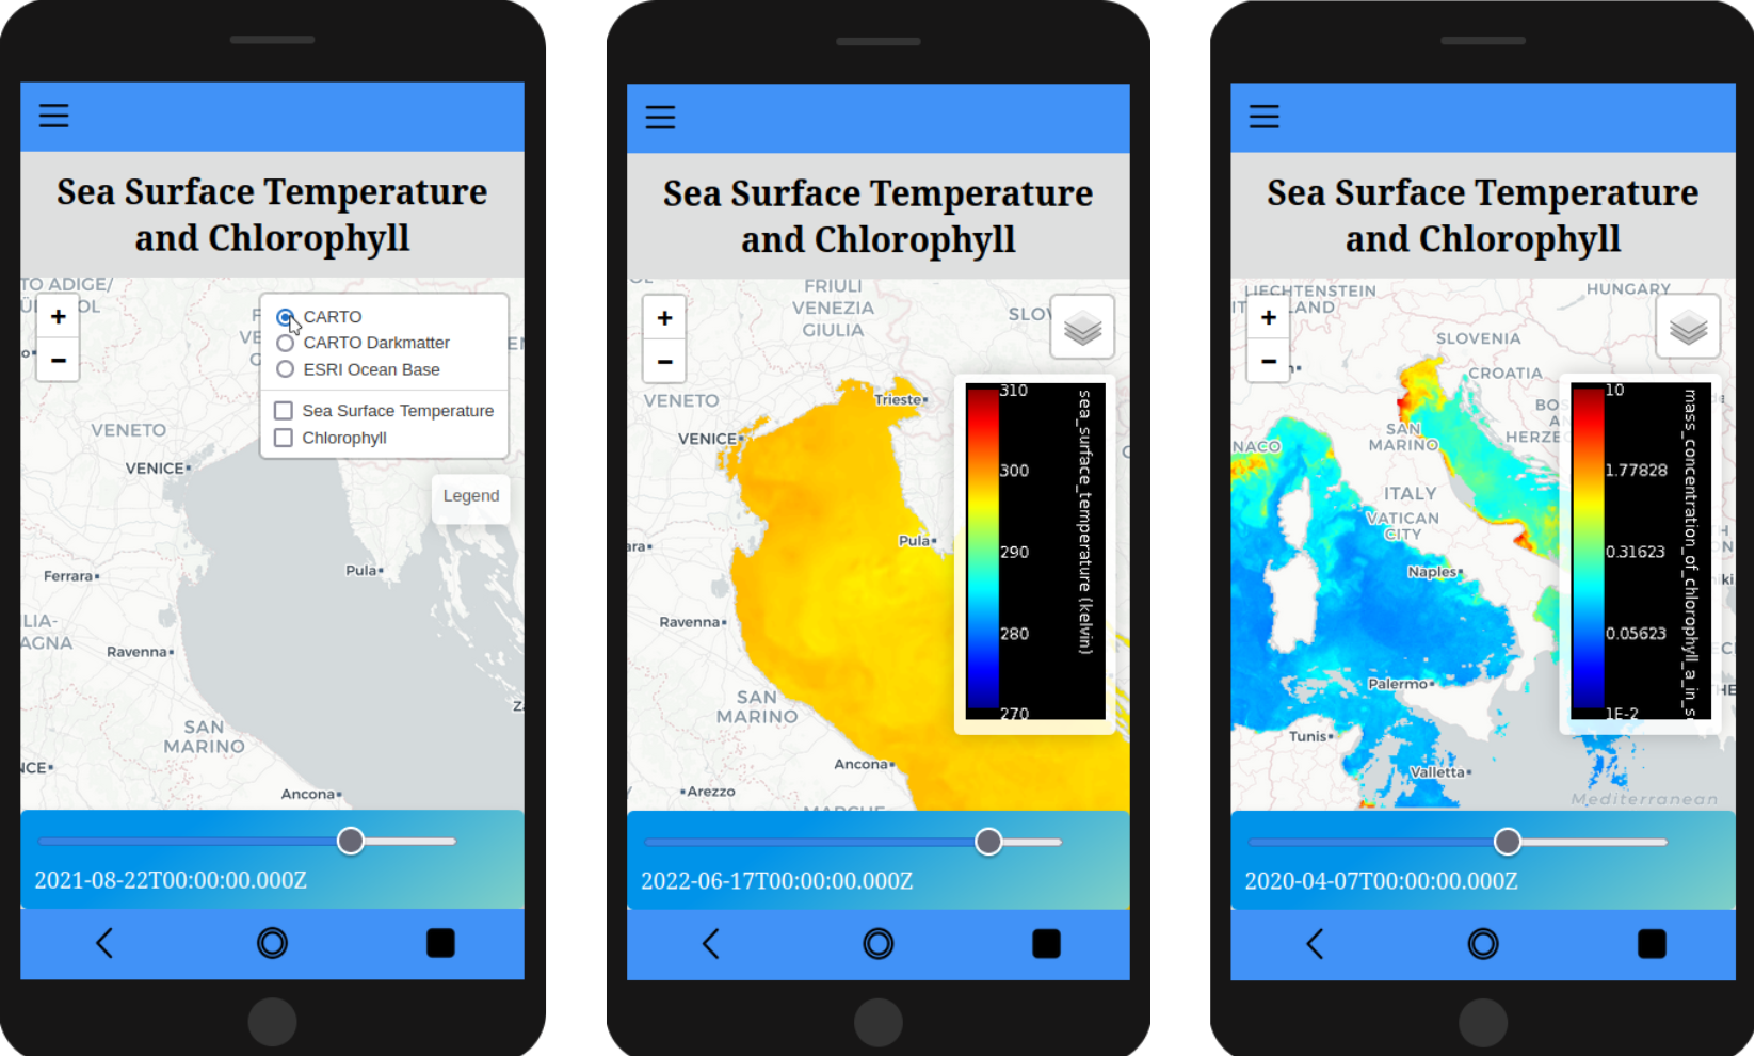
\includegraphics[width=\textwidth]{images/demo_sst_chla.pdf}
\captionsetup{font=small, hypcap=false}
\captionof{figure}{Schermate della demo web che evidenziano il funzionamento dei layer prelevati dal server WMS per temperatura del mare e clorofilla, con relativo posizionamento al di sopra di una mappa base\protect\footnote{Fonte: screenshot dell'autrice.}.}
\label{fig:demo_sst_chla}
\end{minipage}
\hspace{0.05\textwidth}
\vspace{0.25cm}
\end{figure}

La visualizzazione dei dati rilevati dai radar sarà dinamica, tramite un flusso di frecce in movimento ad indicare direzione e velocità del mare. Un esempio, tramite istantanee, è mostrato in \autoref{fig:not_demo_video_plot_radar_30may}.

\begin{figure}[!ht]
\noindent\begin{minipage}[c]{\textwidth}
\vspace{1cm}
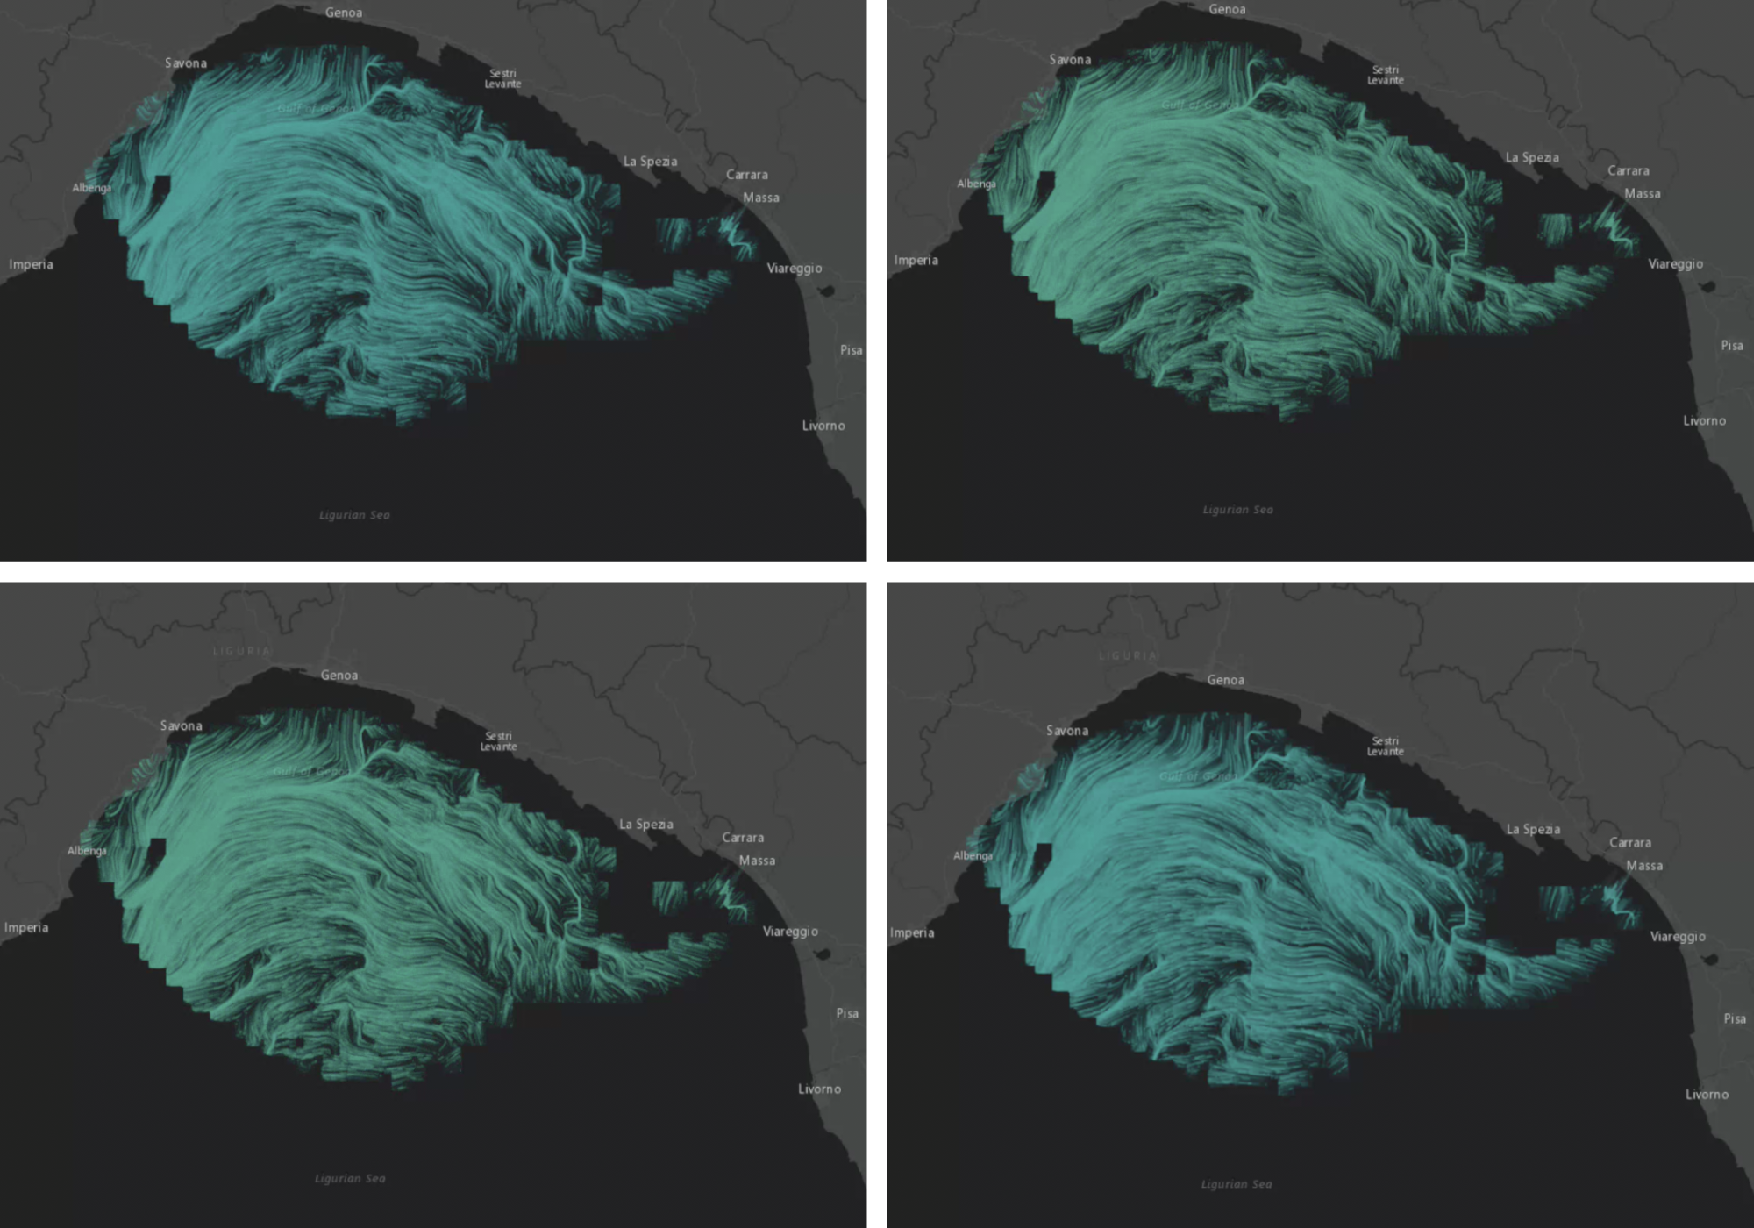
\includegraphics[width=\textwidth]{images/not_demo_video_plot_radar_30may.pdf}
\captionsetup{font=small, hypcap=false}
\captionof{figure}{Istantanee del flusso dei dati rilevati dai radar nella giornata del 30 maggio 2024 alle ore 12:15 (la diversa tonalità di colore viene usata per leggibilità)\protect\footnote{Fonte: screenshot dell'autrice.}.}
\label{fig:not_demo_video_plot_radar_30may}
\end{minipage}
\hspace{0.05\textwidth}
\vspace{0.25cm}
\end{figure}


\paragraph{Sorgenti di dati private.}

La fase di importazione, per le sorgenti private, risulta essere particolarmente critica. Questo deriva dal problema, ampiamente discusso in questa tesi, riguardante la mancanza di dati. È opportuno ricordare che le sorgenti private riguardano i modelli di previsione e le stazioni osservative fisse, escludendo i radar che, come si è visto, hanno dati pubblici in cataloghi thredds. 

Per quanto riguarda i modelli di previsione, quindi Nettuno ed Henetus, il cliente ha fornito dei file contenenti dati di esempio di periodi passati. Non avendo un accesso continuo ai dati non è possibile sviluppare una strategia di import. L'unica funzione sviluppata riguarda la conversione dei file grib di Nettuno in geoTIFF tramite la libreria gdal (vedi \autoref{lst:convert_grib_to_geotiff}), seguendo il modello utilizzato per i cataloghi thredds.

\begin{lstlisting}[language=Python, 
    caption={Definizione funzione per convertire un file grib in geoTIFF.},
    label=lst:convert_grib_to_geotiff]
def convert_grib_to_geotiff(input_file, output_file):
\end{lstlisting}

Invece, per le stazioni osservative fisse, non si è ancora implementata una vera e propria strategia generale di import, perché le uniche variabili disponibili sarebbero le sei della piattaforma Acqua Alta. Per quanto riguarda le altre stazioni, Paloma, S1-GB ed E1, non si è ancora giunti ad un accordo per l'accesso ai dati. Quindi ora saranno analizzate le modalità di accesso alle API, di allMeteo e del comune di Venezia, per le variabili della piattaforma Acqua Alta e la conseguente elaborazione dei dati ottenuti.

Vengono implementate due funzioni differenti per effettuare le richieste alle API di allMeteo (intensità e direzione vento) e del comune di Venezia (livello del mare, altezza d'onda, direzione e intensità del vento).  Quando si fa una richiesta usando l'API allmeteo occorre specificare un token per l'accesso, il sensore da cui prelevare i dati e infine un intervallo di date (vedi funzione in \autoref{lst:fetch_aaot_wind}). 
\begin{lstlisting}[language=python, 
    caption={Definizione funzione per ricavare i dati di intensità e direzione vento dall'api allMeteo.}
    , label=lst:fetch_aaot_wind]
    def fetch_aaot_wind(
        token: str,
        from_time: datetime,
        to_time: datetime,
        devices: List[str] = ["2101LW013"],
    )
\end{lstlisting}

Il risultato sarà lo storico, in formato json, delle misurazioni (effettuate ogni dieci minuti a partire dalle 00:07) nell'arco di tempo specificato. In \autoref{lst:api_allmeteo_res} è presente un esempio dei risultati ottenuti richiedendo i dati dal 28 maggio al 30 maggio 2024 alle ore 00:07 (dai diversi test effettuati si è notato che l'intervallo inizia e termina due ore prima dell'orario specificato). Oltre alla data e ora della misurazione, sono presenti alcune informazioni sul sensore, come il numero di serie, il numero identificativo e il livello di batteria. E poi ci sono i dati reali di intensità del vento (wind\_ave10, wind\_max10, wind\_min10) e la direzione (dir\_ave10, dir\_max10, dir\_hi10, dir\_lo10)
\begin{lstlisting}[language=json, 
    caption={Porzione di storico delle misurazioni di direzione e intensità del vento effettuate nel periodo tra il 28 maggio e il 30 maggio 2024 dal sensore Davis Vantage PRO posto sulla piattaforma Acqua Alta. I dati vengono richiesti all'API allmeteo.}, 
    label=lst:api_allmeteo_res]
[
    {
        "sn": "2101LW013", 
        "timestamp": "2024-05-27 22:07:22", 
        "device_id": 31810, 
        "battery": "4.1",
        "wind_ave10": "0.98950344",
        "wind_max10": "3.742631", 
        "wind_min10": "0",
        "dir_ave10": 336, 
        "dir_max10": 342,
        "dir_hi10": 353,
        "dir_lo10": 319
    },
    {
        "sn": "2101LW013",
        "timestamp": "2024-05-27 22:17:22",
        "device_id": 31810,
        "battery": "4.1",
        "wind_ave10": "1.8389517",
        "wind_max10": "4.164245",
        "wind_min10": "0",
        "dir_ave10": 329,
        "dir_max10": 64,
        "dir_hi10": 65,
        "dir_lo10": 232
    },
    ...
    {
        "sn": "2101LW013",
        "timestamp": "2024-05-29 21:47:23",
        "device_id": 31810,
        "battery": "4.1",
        "wind_ave10": "1.6267841",
        "wind_max10": "5.73184",
        "wind_min10": "0",
        "dir_ave10": 309,
        "dir_max10": 240,
        "dir_hi10": 13,
        "dir_lo10": 245
    }
]
\end{lstlisting}

Nella richiesta alle API del comune di Venezia occorre specificare le credenziali, l'intervallo di date e le variabili d'interesse.  La risposta ottenuta, in formato json, contiene le misurazioni effettuate ogni cinque minuti. La funzione (vedi \autoref{lst:fetch_marea}) che ricava i dati richiede solo il periodo di interesse; la logica dell'accesso tramite credenziali e certificato TLS è implementata all'interno.
\begin{lstlisting}[language=python,
    caption={Definizione funzione per ricavare i dati di livello del mare, altezza d'onda, direzione e intensità del vento.},
    label=lst:fetch_marea]
    def fetch_marea(day_0, day_f)
\end{lstlisting}
In \autoref{lst:api_comuneVE} è presente un esempio dei dati delle quattro variabili (livello del mare, altezza onde, direzione e intensità del vento) nell'intervallo dal 23 maggio al 24 maggio 2024. Se non viene specificata alcuna data si ottengono soltanto le misurazioni effettuate nei 10 minuti precedenti all'orario corrente.

\begin{lstlisting}[language=json, 
    caption={Porzione delle misurazioni di livello del mare, altezza d'onda, direzione e intensità del vento, effettuate nel periodo tra il 23 maggio e il 24 maggio 2024 dai sensori SIAP posti sulla piattaforma Acqua Alta. I dati vengono richiesti all'API del comune di Venezia.}, 
    label=lst:api_comuneVE]
[
    {
        "DATA": "2024-05-23 00:00:00",
        "piattaforma acqua alta siap - livello - metri": "0.56",
        "piattaforma acqua alta siap - onda_altezza_significativa - metri": "0.13",
        "piattaforma acqua alta siap - vento_velocita - m/s": "2.00",
        "piattaforma acqua alta siap - vento_direzione - Gradi": "324.00"
    },
    {
        "DATA": "2024-05-23 00:05:00",
        "piattaforma acqua alta siap - livello - metri": "0.54",
        "piattaforma acqua alta siap - onda_altezza_significativa - metri": null,
        "piattaforma acqua alta siap - vento_velocita - m/s": "1.60",
        "piattaforma acqua alta siap - vento_direzione - Gradi": "311.00"
    },
    {
        "DATA": "2024-05-23 00:10:00",
        "piattaforma acqua alta siap - livello - metri": "0.53",
        "piattaforma acqua alta siap - onda_altezza_significativa - metri": null,
        "piattaforma acqua alta siap - vento_velocita - m/s": "1.50",
        "piattaforma acqua alta siap - vento_direzione - Gradi": "316.00"
    },
    ...
     {
        "DATA": "2024-05-23 23:55:00",
        "piattaforma acqua alta siap - livello - metri": "0.65",
        "piattaforma acqua alta siap - onda_altezza_significativa - metri": null,
        "piattaforma acqua alta siap - vento_velocita - m/s": "4.70",
        "piattaforma acqua alta siap - vento_direzione - Gradi": "236.00"
    },
    {
        "DATA": "2024-05-24 00:00:00",
        "piattaforma acqua alta siap - livello - metri": "0.63",
        "piattaforma acqua alta siap - onda_altezza_significativa - metri": "0.19",
        "piattaforma acqua alta siap - vento_velocita - m/s": "5.00",
        "piattaforma acqua alta siap - vento_direzione - Gradi": "231.00"
    }
]
   
\end{lstlisting}


L'idea dell'import dei dati delle stazioni osservative fisse sarebbe quella di ottenere i dati, elaborarli e salvarli nel database PostgreSQL. Il problema è che, per quanto visto finora, non c'è coerenza tra i dati restituiti dalle API. Inoltre non si sa ancora il formato delle variabili mancanti. Quindi, al momento, viene difficile pensare a una vera e propria strategia per trattare questi dati in modo da uniformarli il più possibile. Ed è il motivo per cui le due API analizzate, al momento, restituiscono semplicemente il file json ricevuto senza un'ulteriore elaborazione.

\end{document}
